\documentclass[]{article}

%opening
\title{}
\author{}

\usepackage{fullpage}
%tikz package 
\usepackage[graphicx]{realboxes}
\usepackage{tikz}
\usetikzlibrary{automata,positioning}

\begin{document}

\begin{figure*}
	\centering
	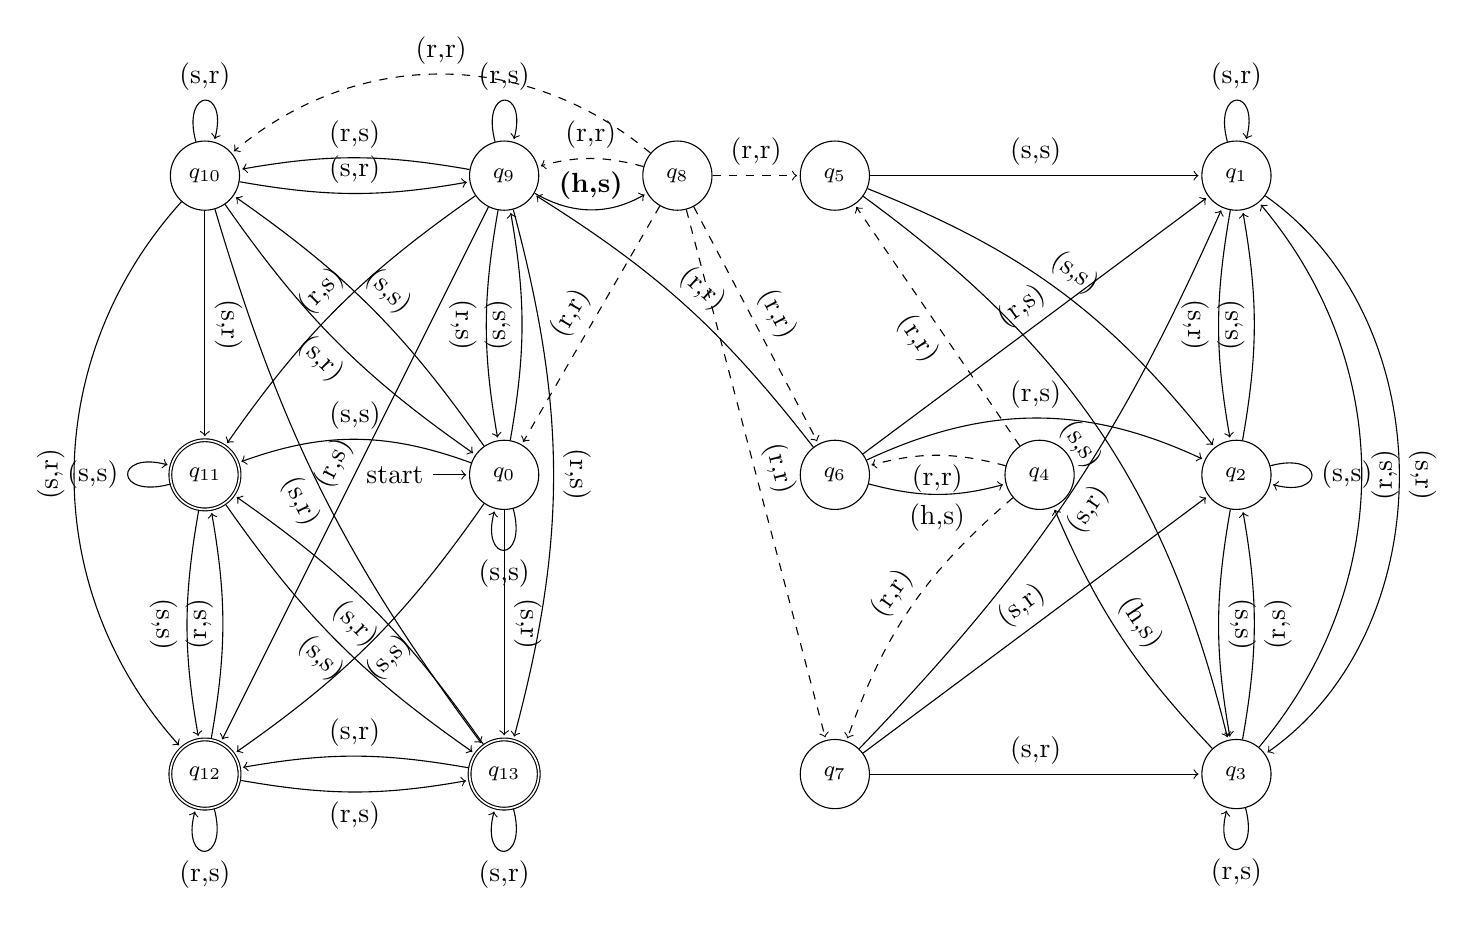
\begin{tikzpicture}[shorten >=1pt,node distance=3.8cm,on grid,auto] 
	\node[state,initial] (q0)   {\footnotesize $q_0$}; 
	\node[state] (q9) [above = of  q0] {\footnotesize $ q_9 $};
	\node[state] (q8) [node distance = 2.2cm] [right = of  q9] {\footnotesize $ q_8 $};
	\node[state] (q5) [node distance = 2cm] [right = of  q8] {\footnotesize $ q_5 $};
	\node[state] (q6) [below = of  q5] {\footnotesize $ q_6 $};
	\node[state] (q7) [below = of  q6] {\footnotesize $ q_7 $};
	\node[state] (q4) [node distance = 2.6cm][right = of  q6] {\footnotesize $ q_4 $};
	\node[state] (q2) [node distance = 2.5cm][right = of  q4] {\footnotesize $ q_2 $};
	\node[state] (q1) [above = of  q2] {\footnotesize $ q_1 $};
	\node[state] (q3) [below = of  q2] {\footnotesize $ q_3 $};
	\node[state] (q10) [left = of  q9] {\footnotesize $ q_{10} $};
	\node[state, accepting] (q11) [left = of  q0] {\footnotesize $ q_{11} $};
	\node[state, accepting] (q12) [below = of  q11] {\footnotesize $ q_{12} $};
	\node[state, accepting] (q13) [below = of q0] {\footnotesize $ q_{13} $};
	\path[->] 
	(q13)   edge [bend right = 10] node [sloped, below] {(s,r)} (q11)
	%s;r;0;;;0;1;0,[13]->[11]
	edge [bend right = 10 ]node [sloped, above] {(s,r)} (q12)
	%   s;r;1;;;0;1;0,[13]->[12]
	edge [loop below ]node  {(s,r)} (q13)
	%   s;r;2;;;0;1;0,[13]->[13]
	(q12)  edge [bend right = 10] node [sloped, above] {(r,s)} (q11)
	%   r;s;0;;;1;0;0,[12]->[11]
	edge [loop below ] node  {(r,s)} (q12)
	%   r;s;1;;;1;0;0,[12]->[12]
	edge [bend right = 10 ]node [sloped, below] {(r,s)} (q13)
	%   r;s;2;;;1;0;0,[12]->[13]
	(q11) edge [loop left]node  {(s,s)} (q12)
	%   s;s;0;;;0;0;0,[11]->[11]
	edge [bend right = 10 ]node [sloped, below] {(s,s)} (q12)
	%   s;s;1;;;0;0;0,[11]->[12]
	edge [bend right = 10 ]node [sloped, below] {(s,s)} (q13)
	%   s;s;2;;;0;0;0,[11]->[13]
	(q10) edge  node [sloped, above] {(s,r)} (q11)
	%   s;r;0;;;0;1;0,[10]->[11]
	edge [bend right = 10]  node  [sloped, below] {(s,r)} (q0)
	%   s;r;0;;;0;1;0,[10]->[0]
	edge [bend right = 42 ]node [sloped, above] {(s,r)} (q12)
	%   s;r;1;;;0;1;0,[10]->[12]
	edge [bend right = 10 ]node [sloped, above] {(s,r)} (q9)
	%   s;r;1;;;0;1;0,[10]->[9]
	edge [bend right = 10] node [sloped, below] {(s,r)} (q13)
	%   s;r;2;;;0;1;0,[10]->[13]
	edge [loop above]node [sloped, above] {(s,r)} ()
	%   s;r;2;;;0;1;0,[10]->[10]
	(q9)  edge [bend right = 30 ]node [sloped, above] {\textbf{(h,s)}} (q8)
	%   h;s;2;;;0;0;0,[9]->[8]
	edge [bend right = 10]node [sloped, above] {(r,s)} (q11)
	%   r;s;0;;;1;0;0,[9]->[11]
	edge [bend right = 10 ]node [sloped, below] {(r,s)} (q0)
	%   r;s;0;;;1;0;0,[9]->[0]
	edge node [sloped, above] {(r,s)} (q12)
	%   r;s;1;;;1;0;0,[9]->[12]
	edge [loop above ]node [sloped, above] {(r,s)} ()
	%   r;s;1;;;1;0;0,[9]->[9]
	edge [bend left = 15 ]node [sloped, above] {(r,s)} (q13)
	%   r;s;2;;;1;0;0,[9]->[13]
	edge [bend right = 10 ]node [sloped, above] {(r,s)} (q10)
	%   r;s;2;;;1;0;0,[9]->[10]
	(q8) edge [dashed]  node [sloped, above] {(r,r)} (q5)
	%   r;r;0;;;2;0;0,[8]->[5]
	edge [dashed] node [sloped, above] {(r,r)} (q0)
	%   r;r;0;;;2;0;0,[8]->[0]
	edge [bend right = 15, dashed ]node [sloped, above] {(r,r)} (q9)
	%   r;r;1;;;2;0;0,[8]->[9]
	edge [dashed] node [sloped, above] {(r,r)} (q6)
	%   r;r;1;;;2;0;0,[8]->[6]
	edge [bend right = 40, dashed ]node [sloped, above] {(r,r)} (q10)
	%   r;r;2;;;2;0;0,[8]->[10]
	edge [dashed] node [sloped, above] {(r,r)} (q7)
	%   r;r;2;;;2;0;0,[8]->[7]
	(q7) edge node [sloped, above] {(s,r)} (q2)
	%   s;r;0;;;0;1;0,[7]->[2]
	edge node [sloped, above] {(s,r)} (q3)
	%   s;r;1;;;0;1;0,[7]->[3]
	edge [bend right = 10]  node [sloped, below] {(s,r)} (q1)
	%   s;r;2;;;0;1;0,[7]->[1]
	(q6) edge [bend right = 15 ]node [sloped, below] {(h,s)} (q4)
	%   h;s;2;;;0;0;0,[6]->[4]
	edge [bend left = 25 ]node [sloped, above] {(r,s)} (q2)
	%   r;s;0;;;1;0;0,[6]->[2]
	edge [bend right = 10 ]node [sloped, above] {(r,r)} (q9)
	%   r;s;1;;;1;0;0,[6]->[3]
	edge node [sloped, above] {(r,s)} (q1)
	%   r;s;2;;;1;0;0,[6]->[1]
	(q5) edge [bend left = 15 ]node [sloped, above] {(s,s)} (q2)
	%   s;s;0;;;0;0;0,[5]->[2]
	edge [bend left = 20 ]node [sloped, below] {(s,s)} (q3)
	%   s;s;1;;;0;0;0,[5]->[3]
	edge node [sloped, above] {(s,s)} (q1)
	%   s;s;2;;;0;0;0,[5]->[1]
	(q4) edge [dashed] node [sloped, below] {(r,r)} (q5)
	%   r;r;0;;;2;0;0,[4]->[5]
	edge [bend right = 15, dashed ]node [sloped, below] {(r,r)} (q6)
	%   r;r;1;;;2;0;0,[4]->[6]
	edge [bend right = 15 , dashed] node [sloped, above] {(r,r)} (q7)
	%   r;r;2;;;2;0;0,[4]->[7]
	(q3) edge [bend left = 10 ]node [sloped, above] {(h,s)} (q4)
	%   h;s;2;;;0;0;0,[3]->[4]
	edge [bend right = 10 ]node [sloped, below] {(r,s)} (q2)
	%   r;s;0;;;1;0;0,[3]->[2]
	edge [loop below ]node  {(r,s)} ()
	%   r;s;1;;;1;0;0,[3]->[3]
	edge [bend right = 40 ]node [sloped, below] {(r,s)} (q1)
	%   r;s;2;;;1;0;0,[3]->[1]
	(q2) edge [loop right]node  {(s,s)} ()
	%   s;s;0;;;0;0;0,[2]->[2]
	edge [bend right = 10 ]node [sloped, above] {(s,s)} (q3)
	%   s;s;1;;;0;0;0,[2]->[3]
	edge [bend right = 10 ]node [sloped, above] {(s,s)} (q1)
	%   s;s;2;;;0;0;0,[2]->[1]
	(q1)  edge [bend right = 10 ]node [sloped, below] {(s,r)} (q2)
	%   s;r;0;;;0;1;0,[1]->[2]
	edge [bend left = 55 ]node [sloped, above] {(s,r)} (q3)
	%   s;r;1;;;0;1;0,[1]->[3]
	edge [loop above]node [sloped, above] {(s,r)} ()
	%   s;r;2;;;0;1;0,[1]->[1]
	(q0) edge [bend right = 20 ]node [sloped, above] {(s,s)} (q11)
	%   s;s;0;;;0;0;0,[0]->[11]
	edge [loop below]node [sloped] {(s,s)} (q9)
	%   s;s;0;;;0;0;0,[0]->[0]
	edge [bend left = 10 ]node [sloped, below] {(s,s)} (q12)
	%   s;s;1;;;0;0;0,[0]->[12]
	edge [bend right = 10 ]node [sloped, above] {(s,s)} (q9)
	%   s;s;1;;;0;0;0,[0]->[9]
	edge node [sloped, above] {(s,r)} (q13)
	%   s;s;2;;;0;0;0,[0]->[13]
	edge [bend right = 10 ]node [sloped, above] {(s,s)} (q10);
	%   s;s;2;;;0;0;0,[0]->[10]
	% 
	%   (q_1)   edge [loop above] node {(s,s,0)} (q_1)
	%           edge  node [sloped, midway]  [below]{(s,s,2)} (q_2)
	%   		   edge  node [sloped, above]{(s,s,1)} (q_3)
	%   (q_2)   edge [loop left] node {(s,r,2)} (q_2)
	%           edge [bend right=20] node [swap] {(s,r,0)} (q_1)
	%      	   edge [bend left = 20] node {(s,r,1)} (q_3)
	%   (q_3)   edge [bend left = 20] node {(r,s,0), (h,s,0)} (q_1)
	%   	       edge [loop below] node {(r,s,1)} (q_3)
	%   	       edge [bend left = 20] node {(r,s,2)} (q_2)
	%   	       edge node [sloped, below] {(h,s,2)} (q_4)
	%   	       edge node [below] {(h,s,1)} (q_5)
	%   (q_4)   edge [bend left = 20, dashed] node [below, sloped] {(r,r,0)}(q_1)
	%           edge [bend right = 20] node [swap]{(h,r,0)}(q_1)
	%           edge [bend left = 20, dashed] node [sloped] {(r,r,1)} (q_3)
	%           edge [bend right = 10] node [sloped, above] {(h,r,1)} (q_3)
	%           edge [dashed] node [sloped, below]{(r,r,2)} (q_2)
	%           edge [bend right = 20 ] node [above, sloped]{(h,r,2)} (q_2)
	%   (q_5)   edge [bend left = 30] node {(r,s,0)} (q_3)
	%           edge [loop below] node {(r,s,1)} ()
	%           edge node [swap, sloped, below]{(r,s,2)} (q_4);
	\end{tikzpicture}
	\caption{All Nash equilibria in Bitcoin Game}
	%\label{Fig:BitcoinNash}
\end{figure*}
\end{document}
	